\paragraph{QuizziPedia::Back-End::App::Controllers::TopicController}
\label{QuizziPedia::Back-End::App::Controllers::TopicController}
\begin{figure}[ht]
	\centering
	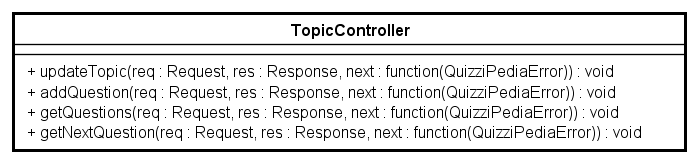
\includegraphics[scale=0.45]{UML/Classi/Back-End/QuizziPedia_Back-End_App_Controllers_topicController.png}
	\caption{QuizziPedia::Back-End::App::Models::Controllers::TopicController}
\end{figure}
\FloatBarrier
\begin{itemize}
	\item \textbf{Descrizione} \\
	Classe che gestisce la logica applicativa riguardante la visualizzazione e la modifica degli argomenti delle domande. È un componente ConcreteHandler del design pattern Chain of responsibility.
	\item \textbf{Utilizzo} \\
	Viene utilizzata per implementare le funzionalità necessarie a gestire le richieste REST legate agli argomenti delle domande.
	\item \textbf{Relazioni con altre classi}
		\begin{itemize}
			\item \textbf{OUT \texttt{TopicModel}} \\
			Classe che modella gli argomenti delle domande.
		\end{itemize}
	\item \textbf{Metodi}
		\begin{itemize}
			\item \texttt{+ updateTopic(req : Request, res : Response, next : function(QuizziPediaError))} \\
			Aggiorna il numero di risposte esatte e totali date a domande sull'argomento da parte degli utenti. \\
			\textbf{Parametri}:
			\begin{itemize}
			\item \texttt{req: Request} \\
			Rappresenta la richiesta inviata al server. Contiene l'identificativo dell'argomento da aggiornare e l'informazione di se è stata data o meno una risposta corretta alla domanda su quell'argomento;
			\item \texttt{res: Response} \\
			Rappresenta la risposta che il server fornirà al termine dell'esecuzione del metodo;
			\item \texttt{next: function(QuizziPediaError)} \\
			Rappresenta la callback che il metodo deve chiamare al termine dell'elaborazione per passare il controllo ai successivi middleware. La presenza del parametro facoltativo QuizziPediaError attiva la catena di gestione dell'errore in sostituzione della normale catena di gestione delle richieste.
			\end{itemize}
			\item \texttt{+ addQuestion(req : Request, res : Response, next : function(QuizziPediaError))} \\
			Aggiunge una domanda tra le domande sull'argomento.  \\
			\textbf{Parametri}:
			\begin{itemize}
			\item \texttt{req: Request} \\
			Rappresenta la richiesta inviata al server. Contiene l'identificativo della domanda creata da un utente e l'identificativo dell'argomento che tratta;
			\item \texttt{res: Response} \\
			Rappresenta la risposta che il server fornirà al termine dell'esecuzione del metodo;
			\item \texttt{next: function(QuizziPediaError)} \\
			Rappresenta la callback che il metodo deve chiamare al termine dell'elaborazione per passare il controllo ai successivi middleware. La presenza del parametro facoltativo QuizziPediaError attiva la catena di gestione dell'errore in sostituzione della normale catena di gestione delle richieste.
			\end{itemize}
			\item \texttt{+ getQuestions(req : Request, res : Response, next : function(QuizziPediaError))} \\
			Restituisce le domande sull'argomento.  \\
			\textbf{Parametri}:
			\begin{itemize}
			\item \texttt{req: Request} \\
			Rappresenta la richiesta inviata al server. Contiene l'identificativo dell'argomento trattato dalle domande che si vuole ottenere;
			\item \texttt{res: Response} \\
			Rappresenta la risposta che il server fornirà al termine dell'esecuzione del metodo;
			\item \texttt{next: function(QuizziPediaError)} \\
			Rappresenta la callback che il metodo deve chiamare al termine dell'elaborazione per passare il controllo ai successivi middleware. La presenza del parametro facoltativo QuizziPediaError attiva la catena di gestione dell'errore in sostituzione della normale catena di gestione delle richieste.
			\end{itemize}
			\item \texttt{+ getNextQuestion(req : Request, res : Response, next : function(QuizziPediaError))} \\
			Restituisce la domanda successiva di un allenamento.  \\
			\textbf{Parametri}:
			\begin{itemize}
			\item \texttt{req: Request} \\
			Rappresenta la richiesta inviata al server. Contiene l'identificativo dell'argomento trattato nell'allenamento e il livello dell'utente che lo sta svolgendo;
			\item \texttt{res: Response} \\
			Rappresenta la risposta che il server fornirà al termine dell'esecuzione del metodo;
			\item \texttt{next: function(QuizziPediaError)} \\
			Rappresenta la callback che il metodo deve chiamare al termine dell'elaborazione per passare il controllo ai successivi middleware. La presenza del parametro facoltativo QuizziPediaError attiva la catena di gestione dell'errore in sostituzione della normale catena di gestione delle richieste.
			\end{itemize}
		\end{itemize}
\end{itemize}